\section{Results and Discussion}

PET has been benchmarked by simulating the test workloads and comparing measured
current drain from the ammeter with the output from PET. This is similar to how
fitness is calculated from the training data sets and their corresponding
measurements in \autoref{sec:multiobjective}.


\subsection{Presentation of Test Sets}

We now present the two test sets used to evaluate PET performance,
\texttt{Dhrystone} and \texttt{Add}.

\subsubsection{Evaluation Set: \texttt{Dhrystone}}

\begin{figure}[H]
\centering
\includegraphics[width=\textwidth]{figs/training/dhrystone-dhry.pdf}
\caption{Overlay of PET training results (red) and training data (green),
\texttt{Dhrystone} test.}
\label{fig:dhry-training}
\end{figure}

The \texttt{Dhrystone} test results drawn in \autoref{fig:dhry-training} is chosen as one
of the final tests for PET as it utilize a wide range of both the integer parts
and memory system of the processors. There is a chance that the values are
weighted wrongly, but still matches the sum of the real power drain. We claim
that decent hits on all four training sets and the Dhrystone test indicates that
the GA found a proper set of weight for the ARM Cortex-A9 processor. Please note
that the y axis in \autoref{fig:dhry-training} starts at $200~mA$, and that the
error is less than $3.9~\%$.


\newpage

\subsubsection{Evaluation Set: \texttt{Add}}

\begin{figure}[ht]
\centering
\includegraphics[width=\textwidth]{figs/training/add-add.pdf}
\caption{Overlay of PET training results (red) and training data (green),
\texttt{Add} test.}
\label{fig:add-training}
\end{figure}

The next test is \texttt{Add}, which is displayed in \autoref{fig:add-training}.
It is particularly interesting because it utilized the fast-loop in the
Cortex-A9. This implies that it would not need its L1-cache nearly as much as
the simulator, as the simulator does not implement fast-loop. However, the real
hardware would keep its ALUs more active than the simulated results, thus PET
will predict a lower power drain, as it thinks that the caches are in use. This
is a problem one must be aware of when the simulator and realized hardware does
not completely correspond to each other. However, the main purpose of PET is to
estimate changes visible at the simulation level. Thus, this is not a real
problem in the ordinary scenarios.


\subsection{Explanations and Errors}

The estimates given by PET is created from a very high level of abstraction, and
will never contain enough information to exactly resemble the power profile of the
realized chip. However, given that the power consuming events are carefully
selected and properly weighted, the current results indicate that this method
works satisfactory.

\begin{figure}[ht]
    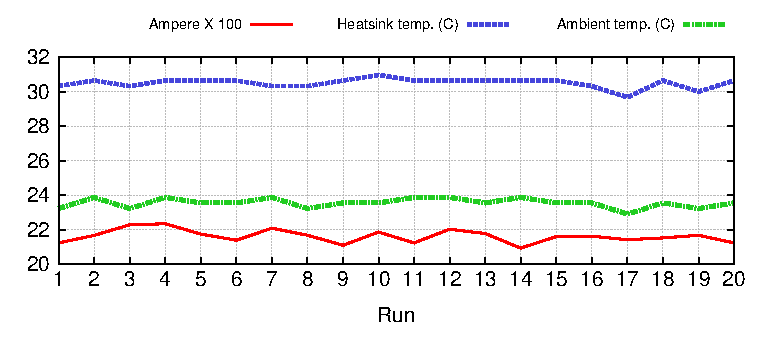
\includegraphics{figs/heat}
    \caption{Variations in measurements.}
    \label{fig:variation}
\end{figure}

In \autoref{fig:variation}, recreated from Figure 8 in
\cite{rundehvatum2013exploring} which uses exactly the same power measurement
setup, it is clear that the measured current drain varies over time seemingly
uncorrelated to both on-chip and ambient temperature. Each data point in the
figure represents the results from a test run of the \texttt{Add} test with
about one hour between each run. The results ranges from $208~mA$ to $224~mA$
and averages to $216~mA$. The results can be written as:
\[
    I_{add} = 216~mA\pm8~mA = 216~mA\pm3.8~\%
\]

With a measured error of $\pm3.8~\%$ it is not unreasonable to expect a $7.6~\%$
error in all measurements. This means that the weights found using measurements
and a GA might be wrong since each training set might have slight discrepancies
between each other. This again renders it impossible to get correct results. By
chance, some genome could fit all training set even though it contains errors,
but the weights would most likely be unequal to the ``correct'' weights.

Most search algorithms are prone to a phenomenon called overfitting
\cite{russellnorvig}. Overfitting happens because the genetic algorithms will
find any kind of obscure patterns in the data sets, e.g., if a high power drain
was seen randomly, but a specific event often happens at that particular time,
the algorithm would try to blame the event for it.

It is clear from \autoref{tbl:gem5runtimeaccuracy} that the CPU model used in
gem5 is not exactly equal to the Cortex-A9 core used in the Samsung
Exynos~4412~Prime SoC, thus each graph in both training and results are
stretched to match each other. This is certainly a source of error, but from
\texttt{Trend} in \autoref{fig:trend-training} and \texttt{SubMul} in
\autoref{fig:submul-training} it is reasonable to believe that the scaling
works, as the change in program flow is shown not far from each other in the
predicted graph and real measurement graph.


\subsection{PET Processing Performance}

To test the performance of PET, we ran a simple benchmark on a system consisting of an
Intel~Core~i7~4820, 32~GB DDR3~SDRAM and reading trace log files from a software
RAID~Level-0 consisting of two Western~Digital Caviar~Black 750~GB disks.

The results shows that reading the trace log file is not the bottleneck, and
that the program itself is CPU-bound. It is easy to feed at least 8~cores when
the log file is hosted on a reasonable fast drive. PET running with 8~threads on
this particular system is consuming log files at a rate of $133~MB/s$,
regardless of whether the log files resides in RAM or on disk. The benchmark used
a log file of $5458~MB$ and took 40.871~seconds to process.

